\documentclass[Deriaz_Traiber_Labo02]{subfiles}


\begin{document}
\chapter{Antenne dipôle}
\section{Objectif}
Le but est de réaliser une antenne qui résonne autour de \SI{2.45}{\giga\hertz}. Le $s_{11}$ à cette fréquence doit être inférieur à \SI{10}{\deci\bel}.


\begin{figure}[H]
\centering
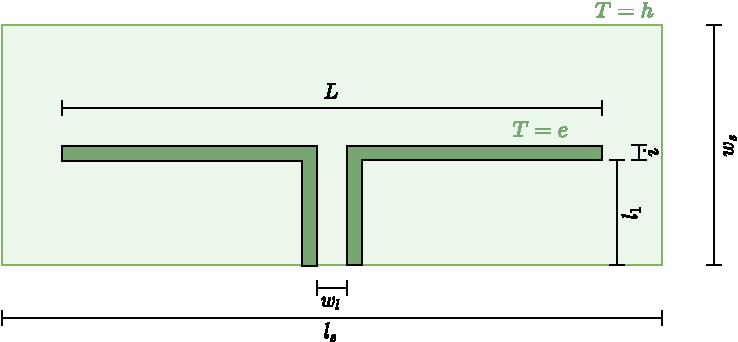
\includegraphics[scale=1,page=1]{../Schemas-crop.pdf}
\caption{Dimensions de l'antenne dipôle}
\end{figure}
\begin{table}[H]
\centering
\begin{tabular}{lll}
\textbf{Variables}\\\hline
$l_1$ & Hauteur du pied\\
$i$ & Épaisseur des brins\\
$L$ & Longueur de l'antenne\\
\textbf{Constantes} & & \textbf{Valeur}\\\hline
$w_l$ & Espacement entre les brins\\
$w_s$ & Largeur du PCB & \SI{30}{\milli\meter}\\
$l_s$ & Longueur du PCB & \SI{80}{\milli\meter}\\
$h$ & Épaisseur du PCB & \SI{1.6}{\milli\meter}\\
$e$ & Épaisseur de cuivre & \SI{35}{\micro\meter}
\end{tabular}
\caption{Liste des dimensions}
\end{table}


\section{FR-4}
La longueur des brins est donnée par l'équation \ref{eq_dipole_longueur}
\begin{equation}
\boxed{L = \dfrac{\lambda}{2\sqrt{\epsilon_r}} = \dfrac{c}{2 f \sqrt{\epsilon_r}}} \Rightarrow \boxed{L = \dfrac{3e8}{2\cdot2.45e9\sqrt{4.3}}=\SI{29.5}{\milli\meter}}
\label{eq_dipole_longueur}
\end{equation}
La dimension du pied est donnée par
\begin{equation}
\boxed{l_1=\frac{\lambda}{8}=\frac{c}{8f}=\SI{15.3}{\milli\meter}}
\end{equation}
La largeur des brins ($i$) a été fixée à \SI{0.8}{\milli\meter} pour le moment.
\subsection{Itérations}
\subsubsection{Première itération}





\section{Céramique}




\subsection{Premier dimensionnement de l'antenne}

Afin de ce familiariser avec le dimensionnement de l'antenne planaire, la méthode utilisé consiste à modifier un seul des paramètres jusqu'à obtenir le résultat le plus proche possible des performances souhaitées puis de réaliser le même démarche pour un second paramètre et ainsi de suite pour les autre paramètre.






\end{document}